\documentclass[a4paper]{article}

\usepackage{amsmath}
\usepackage{amssymb}
\usepackage{parskip}
\usepackage{fullpage}
\usepackage{hyperref}
\usepackage{bettelini}
\usepackage{stellar}
\usepackage{graphicx}
\usepackage{tikz}
\usepackage{fancybox}
\usepackage{makecell}
\usepackage[backend=bibtex]{biblatex}
\usepackage[version=4]{mhchem}

\hypersetup{
    colorlinks=true,
    linkcolor=black,
    urlcolor=blue,
    pdftitle={Chemistry},
    pdfpagemode=FullScreen,
}

\addbibresource{./references.bib}

\title{Chimica}
\author{Paolo Bettelini}
\date{}

\begin{document}

\maketitle
\tableofcontents

% 978.88.08.72527.1
% CHIMICA.BLU J.Brady

\pagebreak

\section{Chimica}

\sdefinition{Sistema}{
    Con \textit{sistema}
    si intende un oggetto o insieme di oggetti isolati
    di cui di studiano le prorpietà termodinamiche.
}

\sdefinition{Ambiente}{
    Con \textit{ambiente} si intende tutto ciò che si
    trova al di fuori del sistema e che è in grado
    di provocare in esso una modifica delle proprietà
    termodinamiche.
}

Sistema \(\subseteq\) Ambiente \(\subseteq\) Universo.

Un sistema può essere:
\begin{itemize}
    \item \textbf{aperto:} se scambia materia/energia con l'ambiente;
    \item \textbf{chiuso:} se scambia solo energia con l'ambiente;
    \item \textbf{osolato:} se non scambia nè energia nè material con l'ambiente.
\end{itemize}

Studiare un sistema significa descrivere le sue proprietà
\begin{itemize}
    \item \textbf{Qualitative:} possono essere definite senza avvalersi
    di misure.
    \item \textbf{Quantitative:} richiedono delle misure.
\end{itemize}
Le priorità misurabili sono delle \textit{grandezze}.

% TODO intensive / estensive

\subsection{Notazione scientifica}

La notazione scientifica viene espressa come
\[
    a \cdot 10^k,\quad a\in [1, 10)
\]

\pagebreak

\subsection{Sistema Internazionale}

\subsubsection{Grandezze fondamentali}

\begin{figure}[h]
    \centering
    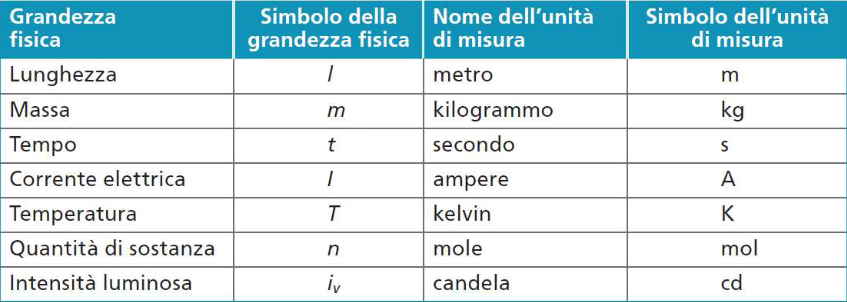
\includegraphics[width=0.75\textwidth]{./si.png}
\end{figure}

\subsubsection{Grandezze derivate}

\begin{figure}[h]
    \centering
    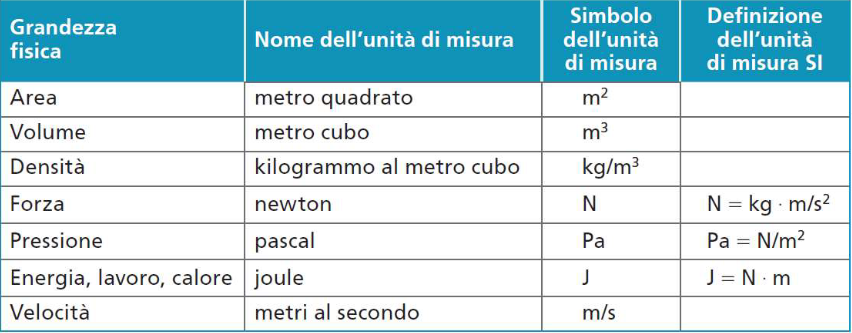
\includegraphics[width=0.75\textwidth]{./grandezzederivate.png}
\end{figure}

\subsubsection{Misure}

\begin{figure}[h]
    \centering
    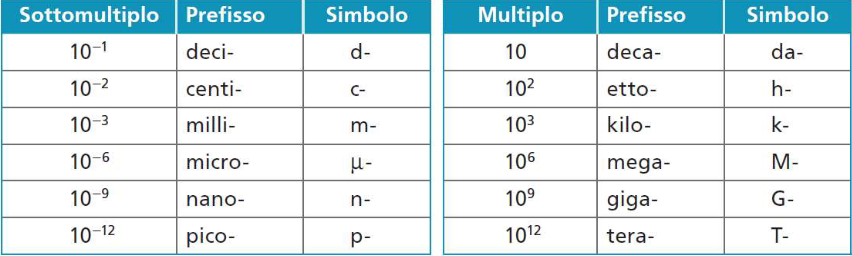
\includegraphics[width=0.75\textwidth]{./misure.png}
\end{figure}

\pagebreak

\section{Trasformazioni}

Le trasformazioni possono essere classificate come \textit{chimiche} o \textit{fisiche}.

\sdefinition{Trasformazione chimica}{
    Una \textit{trasformazione chimica}
    modifica la sostanza.
}

Nelle trasformazioni chimiche, gli atomi sono gli stessi ma gli elementi sono diversi.
Le particelle quindi mutano.

\sdefinition{Trasformazione fisica}{
    Una \textit{trasformazione fisica}
    non modifica la materia ma il suo stato.
}

Nelle trasformazioni fisiche, la materia mantiene le sue proprietà e rimane invariata.

\sexample{Trasformazioni chimiche}{
    \begin{itemize}
        \item Combustione di una candela (anche fisica).
        \item Cottura di un uovo (le proteine cambiano).
        \item Formazione della ruggina.
    \end{itemize}
}

\sexample{Trasformazioni fisica}{
    \begin{itemize}
        \item Combustione di una candela (anche chimica).
        \item Sbucciare una mela.
        \item Scaldare il tisolfato di sofio.
        \item Dissoluzione dello zucchero nell'acqua.
    \end{itemize}
}

\pagebreak

\section{Classificazione}

\subsection{Definizione}

\sdefinition{Sostanza pura elementare}{
    Una \textit{sostanza pura elementare} è composta da un solo tipo di elemento.
}

\sdefinition{Sostanza pura composta}{
    Una \textit{sostanza pura composta} è composta da un solo tipo di composto.
}

\sdefinition{Soluzione}{
    Una \textit{soluzione} è una sostanza composta da diversi tipi di composti
    in maniera omogenea.
}

\sexample{Sostanza pura composta}{
    Acqua (\(H_2O\))
}

\sexample{Sostanza pura elementare}{
    Azoto (\(N\))
}

\sexample{Soluzione}{
    \(50\% N + 50\% H_2\)
}

\begin{center}
    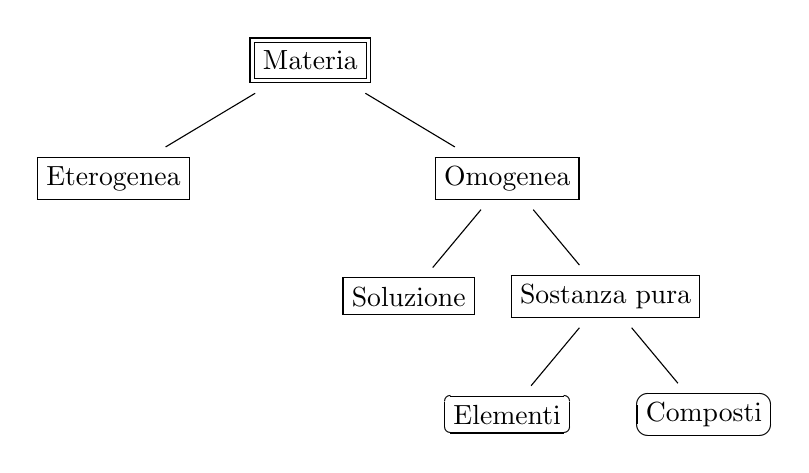
\begin{tikzpicture}[
        level 1/.style = {sibling distance = 5cm},
        level 2/.style = {sibling distance = 2.5cm}
    ]
    \node {\doublebox{Materia}}
        child {
            node {\fbox{Eterogenea}}
        }
        child {
            node {\fbox{Omogenea}}
            child {
                node {\fbox{Soluzione}}
            }
            child {
                node {\fbox{Sostanza pura}}
                child {
                    node {\ovalbox{Elementi}}
                }
                child {
                    node {\ovalbox{Composti}}
                }
            }
        };
    \end{tikzpicture}
\end{center}

\begin{itemize}
    \item La materia può essere classificata come materia \textit{eterogenea}
    e materia \textit{omogenea}.
    
    \item La materia omogenea può essere classificata come \textit{miscuglio omogeneo} (soluzione)
    oppure come \textit{sostanza pura}.
    
    \item Le sostanze pure possono essere classificati come \textit{elementi} oppure \textit{composti}.
\end{itemize}

\pagebreak

\subsection{Soluzioni (miscugli omogenei)}

Ogni soluzione è caratterizzata
da un \textit{soluto} ed un \textit{solvente}.

\sdefinition{Solubilità}{
    La \textit{solubilità} è la quantità massima che una sostanza
    può essere sciolta da una determinata quantità di solvente.
}
La solubilità dipende dalle proprietà chimica e altri fattori come la temperatura.
La solubilità dei gas diminuisce con l'aumento della temperatura.

Una soluzione è detta \textit{satura} o \textit{insatura}
se ha raggiunto il suo quantitativo massimo o meno.

Quando un soluto viene sciolto in un solvente, il volume della soluzione aumenta,
ma meno della somma dei due volumi. Questo è dato dal fatto che il soluto prende spazio fra le molecole del solvente.

\subsection{Tecniche di separazione}

\sdefinition{Decantazione}{
    La \textit{decantazione} si usa di solito per separare due liquidi di densità diversa
    sfruttando la gravità.
}

\sexample{Decantazione}{
    la separazione dell'olio e l'acqua.
}

\sdefinition{Distillazione}{
    La \textit{distillazione} sfrutta i diversi punti di ebollizione di due liquidi per separarli.
    La miscela viene riscaldata fino a quando solo uno delle due componenti diventa vapore, per poi
    spostarla e riaffreddarla.
}

\sdefinition{Cromatografia}{
    La \textit{cromatografia} sfrutta la tendenza delle sostanze a sciogliersi o interagire
    con diverse specie chimiche.
}

\sdefinition{Estrazione}{
    L'\textit{estrazione} si basa sulla maggiore o minore solubilità di un componente di un miscuglio in una certa miscela.
}

\sdefinition{Filtrazione}{
    TODO
}

\sdefinition{Centrifugazione}{
    TODO
}

\pagebreak

%\section{Reazioni chimica}
%Se una reazione chimica fra due elementi ha un rapporto di massa m, il rapporto delle massa atomiche è pari al rapporto, ma contando per il numero di atomi che reagiscono fra di loro.
% Se 1 atomo reasgisce con 1 atomo, il rapporto delle massa del reagente sarà il rapproto delle masse atomiche. 
% Legge delle proporzioni definite e costanti

%\pagebreak


\section{Radioactivity}

\subsection{Definition}

Radioactivity is a set of physical-nuclear processes
through which some unstable or radioactive atomic nuclei decay,
in a certain period of time called decay time.

An unstable nuclei will keep emitting radiations
and transmuting to other nuclei until the atom is stable.

\subsection{Decay}

The mass of a radioactive material will decrease exponentially.

\[
    M(t) = M_0 \cdot e^{-kt}
\]

\(M(t)\) is the mass (or number or particles)
after a certain time \(t\). \(M_0\) is the initial mass
and \(k\) is the rate of decay.

\subsection{Half-life}

The time of half-life is given by \(t_\frac{1}{2} = \frac{\ln 2}{k}\).

\begin{align*}
    \frac{1}{2}M_0 &= M_0 e^{-kt} \\
    \frac{1}{2} &= e^{-kt} \\
    \ln\left(\frac{1}{2}\right) &= -kt \\
    t &= \frac{\ln 2}{k}
\end{align*}

\subsection{Types of radiations}

There are three types of radiations that can be emitted by an unstable nucleai.

\paragraph{\(\alpha\) particles}

An \(\alpha\) particle is a helium nuclei. For example

\[
    \ce{^238_92U -> ^4_2\alpha{} + ^234_90Th}
\]

\paragraph{\(\beta\) particles}

There are two types of \(\beta{}\) particles. \(\beta{}^+\) and \(\beta{}^-\).
A \(\beta{}^+\) particle is emitted when the nuclei is unstable due to
having too many protons, whist the \(\beta{}^-\) one is emitted when it has
too many neutrons.

\[
    \begin{cases}
        \beta{}^+,\quad \ce{^0_{+1}e} \text{ (positron)} \\
        \beta{}^-,\quad \ce{^0_{-1}e} \text{ (electron)}
    \end{cases}
\]

\paragraph{\(\gamma\) particles}

\(\gamma\) rays are photons of electromagnetic energy. They have \(0\) mass and \(0\) charge.

\pagebreak

\section{Energy levels}

An electron is a fundamental particle. It is attracted by protons in the
atom nuclei but they repelled by one another.
The places where the electrons are found around the nuclei are called
\textit{atomic orbitals.} \\
There are two types of orbitals, \textbf{s} and \textbf{p}.
Electrons in \textbf{s} orbitals can be measured to be in a spherical region around the nuclei,
whilst electrons in \textbf{p} orbitals have a dumbell-shaped position region
(zero-probability of being measured at the center of the nuclei).
An orbital can host up to two electrons.
Orbitals are grouped in different zones.
Eletrons in zones closer to the center have lower energy and the amount of energy
to move an electron from its zone to the next one is constant.

At the lower energy there is a single \(1\text{s}\) orbital that can hold two electrons.
At the next energy level, there are four orbitals:
\(2\text{s}\), \(2\text{p}1\), \(2\text{p}2\) and \(2\text{s}3\) for up to 8 electrons at this level of energy.
In larger atoms electrons can be found at the level \(3\text{s}\) and \(3\text{p}\)

Atoms where the level with most energy is not completly empty or completly full is unstable.
The excess electorns are called valence electrons. An atom may share, give or take electrons
with other atoms to become stable.

\subsection{Ionic bond}

An ionic bond is a transfer of valence electrons between metallic atoms and non-metallic atoms.
The outcome of this process is a positive ion (more protons than electrons)
and a negative ion (more electrons than protons). These ions attract each other often
forming a crystal structure.

\subsection{Metallic bond}

A metallic bond is a transfer of valence electrons between metallic atoms.
The valence electrons continually move from one atom to another and are not
associated with any specific pair of atoms. This creates a structure of positive ions
which conducts electricity (since electrons can freely move).

\subsection{Covalent bond}

A covalent bond is a sharing of pairs of electrons between non-metallic atoms.
A covalent bond happens just between two atoms, it can be simple, double or triple (2, 4, 6 total shared electrons).

\subsection{Electronegativity}

Electronegativity is a measure of an atom's ability to attract shared electrons to itself.
The type of bond if given by the different of electronegativity between two atoms.
\begin{itemize}
    \item \(0\) - \(0.4\): Pure covalent bond
    \item \(0.4\) - \(1.7\): Polar covalent bond
    \item \(1.7\) -: Ionic bond
\end{itemize}

\pagebreak

\section{Acids}

The pH level is a measure of the acidity or alkalinity of a solution. It is a logarithmic scale that ranges from 0 to 14, with 7 being considered neutral. A pH value below 7 indicates acidity, while a pH value above 7 indicates alkalinity.

The pH scale is based on the concentration of hydrogen ions (\(\text{H}^+\)) in a solution. An acidic solution has a higher concentration of \(\text{H}^+\) ions, while an alkaline solution has a lower concentration of \(\text{H}^+\) ions. The pH scale is logarithmic..

OH stands for hydroxide ion, which is a negatively charged molecule consisting of one oxygen atom and one hydrogen atom. It is the conjugate base of water (\(\text{H}_2\text{O}\)) and plays a role in determining the pH level of a solution. The concentration of \(\text{OH}^-\) ions in a solution is directly related to its alkalinity, as the higher the concentration of \(\text{OH}^-\) ions, the more alkaline the solution is.

\begin{align*}
    \text{pH} &= - \log_{10}(\text{H}^+) \\
    \text{pOH} &= - \log_{10}(\text{OH}^-) \\
    \text{pH} + \text{pOH} &= 14 \\
\end{align*}

\pagebreak

\section{Redox}

\subsection{Definition}

Redox (reduction-oxidation) reactions are a chemical reaction in which electrons are transferred between two reactants participating in it.
A redox reaction involves a change in the oxidation state of one or more atoms.
Whoever loses electrons is oxidized, whilst whoever gains electrons is reduced.

\subsection{Oxidation State}

The oxidation state or odixation number of an atom in a molecule represents its ability to lose or gain electrons in a chemical reaction. In a neutral molecule, the sum of the oxidation states of all atoms is always equal to zero. This means that the sum of the electrons lost by some atoms is equal to the sum of the electrons gained by other atoms.

\begin{enumerate}
    \item Individual elements always have an oxidation number of \(0\).
    \item Monoatomic ions always have an oxidation number of \(0\).
    \item Hydrogen (\textit{almost}) always has an oxidation number of \(+1\).
    \item Oxygen (\textit{almost}) always has an oxidation number of \(-2\).
\end{enumerate}

If the oxidation state increases, the molecule oxidises (loses electrons). \\
If the oxidation state decreases, the molecule reduces (gains electrons).

\subsection{Spontaneous reactions}

A reaction is \textit{spontaneous} if it proceeds spontaneously.

%i metalli dei primi gruppi tendono a cedere i propri elettroni esterni OSSIDANDOSI;

%i non metalli, molto elettronegativi, acquistano invece elettroni, RIDUCENDOSI;

\pagebreak

\section{Polarità}

\sdefinition{Polarità}{
    Una molecola è polare (non pura) se vi è una carica parziale.
}
Il legale ionico è quello più polare perché strappa un elettrone. \\
La differenza di elettronegatività deve essere da 0 a 0.45 per essere puro
(il valore 0.45 è scelto per considerare il legame CH come apolare).

Quando una molecola è fatta solo da 2 atomi, 
se il legame è polare, la molecola è polare.
Quando ci sono più legami, è necessario almeno un legame polare
ma la molecola non deve essere simmetrica, altrimenti le cariche parziali si annullano.

Le sostanze apolari si sciolgono in solventi apolari, e quelli polari in quelli polari.
Di conseguenza, oer essere solubile in acqua una moecola deve essere polare.


\section{Lgami secondari (forze intermolecolari)}

\sdefinition{Forza forte}{
    Legame covalente, metallico o ionico.
}
\sdefinition{Forza debole}{
    Forze di Van der Walls, forze di Londom, ponte a idrogeno.
}

I legami secondari (deboli, intermolecolari) sono responsabili delle interazioni fra molecole uguali o diverse tra loro,
o anche fra parti diverse della stessa molecola.

Se il legame non è un ponte idrogeno ma è lo stesso principio, di dice dipolo-dipolo.
Infatti, il legame ponte idrogeno è dipolo-dipolo ma ha un nome speicfico.
Le forze di Van der Walls sono i legami dipolo-dipolo.
Quando le interazioni non sono polari si parla di forze di London.

\subsection{Dissoluzione del sale nell'acqua}

L'acqua ed il sale Na\(^{+}\)Cl\(^{-}\) inducono un polo.
Le cariche positive dell'acqua (idrogeno) vengono attratte da quelle negative
del cloruro, mentre quelle negative dell'acqua (ossigeno)
vengono attratti da quelle negative del sale (Na).
Il cristallo del sale viene quindi separato dalle forze
esercitate dai dipoli dell'acqua.

Il motivo per cui il cristallo si spacca e non le molecole di acqua
è dato dal fatto che l'energia delle interazioni deboli è più che sufficiente
per compensare l'energia necessaria per rompere le interazioni ione-ione
nel cristallo e alcuni legami idrogeno acqua-acqua.

\subsection{Forze deboli nell'H2O}

I ponti a idrogeno creano una struttura esagonale con le molecole d'acqua,
formando il ghiaccio.
Questo è il motivo per cui la struttura dei giocchi di neve è esagonale.
Quando l'acqua è gassosa non ci sono queste forze debole, e quando sono
liquide ce ne sono poche e casuali.
Il motivo è che l'energia aumuenta con l'aumentare della temperatura,
e per cui con temperature troppe alte, questa energia spacca i legami deboli.

Il sale nell'acqua salata rende più difficile la creazione di ponti a idrogeno.

% anche il motivo per cui l'acqua ghiaccia solo sopra
% foto esagono e fiocchi di neve

\pagebreak

\subsection{Sviluppo del calore nelle reazioni}

La rottura di un legame necessita di energia, mentre
la formazione di legami libera energia.

\begin{center}
\begin{figure}[h]
    \centering
    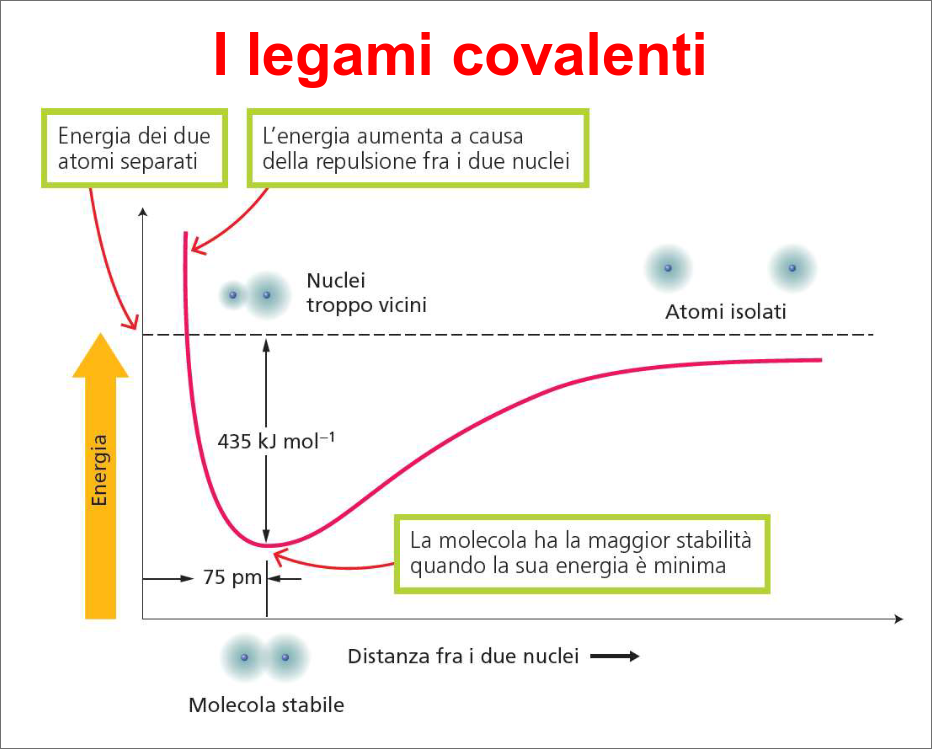
\includegraphics[width=\textwidth]{./cov_bond_energy.png}
\end{figure}
\end{center}

\sdefinition{Entalpia}{
    L'\textit{entalpia} è la quantità di energia interna che un sistema
    termodinamico può scambiare con l'ambiente.
}

\sdefinition{Reazione esotermica}{
    Una \textit{reazione esotermica} è una reazione che libera energia termica.   
}

La reazione esotermica possiede le seguenti caratteristiche:
\begin{itemize}
    \item la reazione rilascia calore;
    \item l'ambiente circostance si scalda;
    \item l'entalpia \(\Delta H_{\text{reazione}} < 0\);
    \item i legami che si formano nei prodotti sono più forti di quelli che si rompono nei reagenti;
    \item i prodotti hanno energia inferiore rispetto ai reagenti.
\end{itemize}

\sdefinition{Reazione endotermica}{
    Una \textit{reazione endotermica} è una reazione che assorbe energia termica.   
}

La reazione esotermica possiede le seguenti caratteristiche:
\begin{itemize}
    \item l'entalpia \(\Delta H_{\text{reazione}} > 0\);
\end{itemize}

In una reazione esotermica all'equilibrio chimico,
aumentando la temperatura si sposta tale equilibrio verso i reagenti,
per cui la reazione inversa è favorita rispetto alla reazione diretta
per temperature elevate. Il segno della variazione di entalpia
(che è un aspetto termodinamico) indica semplicemente la predisposizione della
reazione chimica ad evolversi in senso diretto o inverso,
mentre per conoscere la velocità di reazione è necessario considerare gli aspetti cinetici.

L'energia è direttamente proporzionale alle mole, e quindi alla massa.

Il calore acquisito o rilasciato da un corpo è durettamente proporzionale
alla variazione di temperatura a cui va incontro e si ricava dall'espressione
\[
    Q = mc\Delta T
\]
dove \(c\) è il calore specifico.

\sdefinition{Entalpia standard di formazione}{
    L'\textit{entalpia standard di formazione}
    di una sostanza, o \textit{calore standard di formazione}
    è la quantità di calore assorbita o liberata quando una mole della sostanza
    viene formata, a \(25 {}^\circ \) C e 1 atm, dai suoi elementi nei loro stati standard.
}

Conoscendo l'entalpia delle sostanze, per qualunque
reazione possiamo calcolare direttamente la variazione di energia di reazione.
\[
    \Delta H^\circ_{\text{reazione}} =
    \sum_{f \in \text{reazione}} \left( \Delta H^\circ_f \right) -
    \sum_{f \in \text{reagenti}} \left( \Delta H^\circ_f \right) 
\]

L'Entalpia Standard di Formazione,
\(\Delta H^\circ_f\), di una sostanza è il \(\Delta H^\circ\)
della sua reazione di formazione.

Una sostanza pura ha sempre entalpia di formazione \(\Delta H^\circ_f = 0\).

\pagebreak

\section{Isotopi dell'idrogeno}

\subsection{Deuterio}

Il primo isotopo dell'idrogeno è il \textit{deuterio}, indicato con \(D\) o \(^2H\).
A differenza dell'idrogeno comune, il deuterio possiede un neutrone nel nucleo oltre al protone.
A causa di questa caratteristica, il deuterio ha una massa atomica leggermente superiore rispetto all'idrogeno normale.
Il deuterio è utilizzato in varie applicazioni, come nei reattori nucleari per la produzione di energia e come tracciatore in studi scientifici e biologici. 

\subsection{Trizio}

Il secondo isotopo dell'idrogeno è è il trizio, indicato con \(T\) o \(^3H\).
A differenza dell'idrogeno comune, il deuterio possiede due neutroni nel nucleo oltre al protone.
A causa di questa composizione nucleare, il trizio ha una massa atomica maggiore rispetto agli altri isotopi dell'idrogeno.
Il trizio è radioattivo e decade nel tempo con una emivita di circa 12,3 anni, emettendo particelle beta.

\section{Acqua con deuterio e trizio}

È possibile ottenere dell'acqua, \(H_2O\), utilizzando gli isotopi \(D\) e \(T\) al posto di \(H\).

Queste sostanze sono chiamate \textit{acqua pesante} (\(D_2O\)) e
\textit{acqua superpesante} (\(T_2O\)).

\subsection{Densità}

\begin{center}
    \bgroup{}
    \def\arraystretch{1.25}
    \begin{tabular}{ |c|c|c|c| }
        \hline
        & \textbf{Acqua} & \textbf{Acqua pesante} & \textbf{Acqua Superpesante} \\
        \hline
        \textbf{Liquido (g/cm\(^3\))} & 0.997 & 1.11 & 1.20 \\
        \hline
        \textbf{Solido (g/cm\(^3\))} & 0.9168 & 1.105 & ? \\
        \hline
    \end{tabular}
    \egroup{}
\end{center}

Normalmente, le molecole dell'acqua che ghiaccia si organizzano, e creano molti spazi (caso unico).
Questo implica che il ghiaccio abbia una densità minore dell'acqua, per cui esso galleggia se immerso nell'acqua.

Possiamo quindi notare dalla tabella come la versione solida dell'acqua pesante galleggi
nell'acqua normale \cite{deuterated-water}.

\nocite{*} % cite all entries

\printbibliography

% reagenti -> prodotti + E (eso)
% reagenti + E -> prodott (endo)

\end{document}

APPUNTI ESPE:
Fare frasi complete con la maiuscola
Nell'esercizio scrivere i passaggi con le unità di misura in maniera sequenziale.
I risultati metteteli in una frase: es. si sono prodotti 5g di merda